% Imporditud: tools/import_eksperimendid.py
% Allikas: Eesti füüsikaolümpiaadi eksperimendi ülesannete
%   kogu (Rael Kalda, 2023), ülesanne Ü170, lahendus L170.
\setAuthor{EFO žürii}
\setRound{lõppvoor}
\setYear{2012}
\setNumber{G E1}
\setDifficulty{5}
\setTopic{elektriahelad}
\setVahendid{uuritav seade, tester. Testri tootja poolt lubatav mõõtemääramatus oommeetrina on kirjutatud eraldi lehele töölaual. Pange tähele, et antud on mittelineaarne potentsiomeeter: ka lahtiühendatuna ei sõltu takistus potentsiomeetri liuguri ja otsa vahel nupu pöördenurgast lineaarselt. Siiski, liugurid jaotavad potentsiomeetrite takistused alati sama suurteks osadeks}
\setPunktid{12}
\setAllikas{Eksperimendi kogu Ü170, lahendus lk 128}
\setLahendusseis{toores}

\prob{Stereopotentsiomeeter}
Karbis on ühisel teljel kaks ühesugust potentsiomeetrit, mis on ühendatud nagu skeemil. Seadme nupu keeramisel nihkuvad potentsiomeetrite liugkontaktid samal määral ja joonisel samas suunas. Karbist on välja toodud skeemil näidatud juhtmeotsad. Leidke ühe potentsiomeetri äärmiste klemmide vaheline takistus, mis tal oleks lahtiühendatuna. Hinnake mõõtemääramatust.
\begin{center}
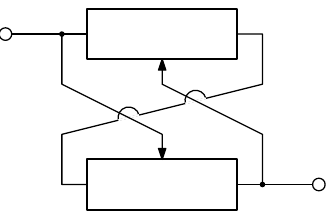
\includegraphics[width=0.28\linewidth]{2012-v3g-ge1-yl.png}
\end{center}

\hint

\solu
Keerame uuritava seadme juhtmeotsad kindlalt oommeetri omade ümber. Mõõda-(1 $- \alpha$)R me takistust juhtmeotste vahel ning keerame nuppu. Oommeetri näidul on nupu pöördenurga funktsioonina ainult üks maksimum. Et nii on, teeme kindlaks kas katseliselt (mis on lihtsam) või arvutuslikult. Arvutuslikus lähenemises väljendagu liuguri asendit parameeter $\alpha$ (mis sõltub nupu pöördenurgast mittelineaarselt, aga see polegi oluline) nii, et mõlemat potentsiomeetrit võib käsitleda kui (1 $- \alpha$)R $\alpha$R

128 $\alpha$R

ühendust $\alpha$R (1 $- \alpha$)R . Siis on seadme kogutakistus arvutatav

paremal toodud ekvivalentskeemi järgi:

1 ( 1 )

Rseade = 1 + 1 + 1 =R 1 $- \alpha$(1 $- \alpha$) + 1 . $\alpha$R+(1$-\alpha$)R $\alpha$R (1$-\alpha$)R

1 on positiivse ruutfunktsiooni pöördväärtus, mil on muidugi ainult üks $\alpha$(1$-\alpha$)+1

miinimum. Paneme veel tähele, et avaldis on sümmeetriline $\alpha$ ja (1$-\alpha$) vahetamise

suhtes, mistõttu on mõõdetava takistuse maksimum parajasti kohas, kus $\alpha$ = 1 ehk liugur jagab potentsiomeetri takistuse pooleks.

Olles teinud kindlaks, et maksimume on vaid üks, saanuks sa-

ma järelduse, et see asub kohas, kus liugurid poolitavad po- R/2

tentsiomeetrite takistused, ka otse skeemi sümmeetriale tugine-

des: skeemi 180 pöörates peab mõõdetav takistus samaks jääma R/2 R/2

ja maksimum peab sellel pöördel teisenema iseendaks. Sellises

sümmeetrilises olukorras on meil paremal toodud ekvivalents- R/2

keem, mille takistus on (analoogiliselt ülalkirjutatud arvutusega)

R/5.

Niisiis peame vastuse saamiseks mõõtma suurima võimaliku ta-

kistuse ja korrutama selle viiega. Testrinäitude hajumine fikseeritud takistuse

mõõtmisel on minimaalne, seega kordusmõõtmistest on kasu vaid niivõrd, kuni

need aitavad suuremat maksimumväärtust leida. Nende tulemusi keskmistada on

antud katses vale, kuna teame, et (õige mõõtmistehnika juures) ei saa juhusli-

kult õigest suuremat takistust mõõta. Küll tuleb olla tähelepanelik, et iseennast

mitte vooluringi ühendada: kätevaheline takistus võib mõõdetavaga samas suu-

rusjärgus või mitu korda väiksemgi olla! Realistlik vastus on sõltuvalt konkreet-

sest katseseadmest ligikaudu 370...550 k$\Omega$ (potentsiomeetri nominaalväärtus oli

470 k$\Omega\pm$20\%; kõrvalekaldeid lisas fakt, et ühesuguste potentsiomeetrite paarisole-

mise eeldus polnud tegelikult täpne).

Määramatusehinnaguna on põhiline oommeetri enda määramatus kasutatavas mõõ-

tepiirkonnas. Kui maksimumi otsimiseks oleks rangelt dokumenteeritud ja ma-

sinlikult järgitud algoritm, saaks selle vahetulemuste järgi ka hinnata, kui täpselt

nupp maksimumtakistuse juurde keerati, ning sealtkaudu leida lisaks statistilise

määramatuse ning (mitte keskmistades!) täpsema tõelise maksimumi hinnangu,

aga ainuüksi antud vahenditega seda teha ei saa.
\probend
